% A LaTeX template for MSc Thesis submissions to 
% Politecnico di Milano (PoliMi) - School of Industrial and Information Engineering
%
% S. Bonetti, A. Gruttadauria, G. Mescolini, A. Zingaro
% e-mail: template-tesi-ingind@polimi.it
%
% Last Revision: October 2021
%
% Copyright 2021 Politecnico di Milano, Italy. NC-BY

\documentclass{Configuration_Files/PoliMi3i_thesis}
\usepackage{algorithm}
%------------------------------------------------------------------------------
%	REQUIRED PACKAGES AND  CONFIGURATIONS
%------------------------------------------------------------------------------

% CONFIGURATIONS
\usepackage{parskip} % For paragraph layout
\usepackage{setspace} % For using single or double spacing
\usepackage{emptypage} % To insert empty pages
\usepackage{multicol} % To write in multiple columns (executive summary)
\setlength\columnsep{15pt} % Column separation in executive summary
\setlength\parindent{0pt} % Indentation
\raggedbottom  

% PACKAGES FOR TITLES
\usepackage{titlesec}
% \titlespacing{\section}{left spacing}{before spacing}{after spacing}
\titlespacing{\section}{0pt}{3.3ex}{2ex}
\titlespacing{\subsection}{0pt}{3.3ex}{1.65ex}
\titlespacing{\subsubsection}{0pt}{3.3ex}{1ex}
\usepackage{color}

% PACKAGES FOR LANGUAGE AND FONT
\usepackage[english]{babel} % The document is in English  
\usepackage[utf8]{inputenc} % UTF8 encoding
\usepackage[T1]{fontenc} % Font encoding
\usepackage[11pt]{moresize} % Big fonts

% PACKAGES FOR IMAGES
\usepackage{graphicx}
\usepackage{transparent} % Enables transparent images
\usepackage{eso-pic} % For the background picture on the title page
\usepackage{subfig} % Numbered and caption subfigures using \subfloat.
\usepackage{tikz} % A package for high-quality hand-made figures.
\usetikzlibrary{}
\graphicspath{{./Images/}} % Directory of the images
\usepackage{caption} % Coloured captions
\usepackage{xcolor} % Coloured captions
\usepackage{amsthm,thmtools,xcolor} % Coloured "Theorem"
\usepackage{float}

% STANDARD MATH PACKAGES
\usepackage{amsmath}
\usepackage{amsthm}
\usepackage{amssymb}
\usepackage{amsfonts}
\usepackage{bm}
\usepackage[overload]{empheq} % For braced-style systems of equations.
\usepackage{fix-cm} % To override original LaTeX restrictions on sizes

% PACKAGES FOR TABLES
\usepackage{tabularx}
\usepackage{longtable} % Tables that can span several pages
\usepackage{colortbl}

% PACKAGES FOR ALGORITHMS (PSEUDO-CODE)
\usepackage{algorithm}
\usepackage{algorithmic}

% PACKAGES FOR REFERENCES & BIBLIOGRAPHY
\usepackage[colorlinks=true,linkcolor=black,anchorcolor=black,citecolor=black,filecolor=black,menucolor=black,runcolor=black,urlcolor=black]{hyperref} % Adds clickable links at references
\usepackage{cleveref}
\usepackage[square, numbers, sort&compress]{natbib} % Square brackets, citing references with numbers, citations sorted by appearance in the text and compressed
\bibliographystyle{abbrvnat} % You may use a different style adapted to your field

% OTHER PACKAGES
\usepackage{pdfpages} % To include a pdf file
\usepackage{afterpage}
\usepackage{lipsum} % DUMMY PACKAGE
\usepackage{fancyhdr} % For the headers
\fancyhf{}

% Input of configuration file. Do not change config.tex file unless you really know what you are doing. 
% Define blue color typical of polimi
\definecolor{bluepoli}{cmyk}{0.4,0.1,0,0.4}

% Custom theorem environments
\declaretheoremstyle[
  headfont=\color{bluepoli}\normalfont\bfseries,
  bodyfont=\color{black}\normalfont\itshape,
]{colored}

% Set-up caption colors
\captionsetup[figure]{labelfont={color=bluepoli}} % Set colour of the captions
\captionsetup[table]{labelfont={color=bluepoli}} % Set colour of the captions
\captionsetup[algorithm]{labelfont={color=bluepoli}} % Set colour of the captions

\theoremstyle{colored}
\newtheorem{theorem}{Theorem}[chapter]
\newtheorem{proposition}{Proposition}[chapter]

% Enhances the features of the standard "table" and "tabular" environments.
\newcommand\T{\rule{0pt}{2.6ex}}
\newcommand\B{\rule[-1.2ex]{0pt}{0pt}}

% Pseudo-code algorithm descriptions.
\newcounter{algsubstate}
\renewcommand{\thealgsubstate}{\alph{algsubstate}}
\newenvironment{algsubstates}
  {\setcounter{algsubstate}{0}%
   \renewcommand{\STATE}{%
     \stepcounter{algsubstate}%
     \Statex {\small\thealgsubstate:}\space}}
  {}

% New font size
\newcommand\numfontsize{\@setfontsize\Huge{200}{60}}

% Title format: chapter
\titleformat{\chapter}[hang]{
\fontsize{50}{20}\selectfont\bfseries\filright}{\textcolor{bluepoli} \thechapter\hsp\hspace{2mm}\textcolor{bluepoli}{|   }\hsp}{0pt}{\huge\bfseries \textcolor{bluepoli}
}

% Title format: section
\titleformat{\section}
{\color{bluepoli}\normalfont\Large\bfseries}
{\color{bluepoli}\thesection.}{1em}{}

% Title format: subsection
\titleformat{\subsection}
{\color{bluepoli}\normalfont\large\bfseries}
{\color{bluepoli}\thesubsection.}{1em}{}

% Title format: subsubsection
\titleformat{\subsubsection}
{\color{bluepoli}\normalfont\large\bfseries}
{\color{bluepoli}\thesubsubsection.}{1em}{}

% Shortening for setting no horizontal-spacing
\newcommand{\hsp}{\hspace{0pt}}

\makeatletter
% Renewcommand: cleardoublepage including the background pic
\renewcommand*\cleardoublepage{%
  \clearpage\if@twoside\ifodd\c@page\else
  \if@twocolumn\hbox{}\newpage\fi\fi\fi}
\makeatother

%For correctly numbering algorithms
\numberwithin{algorithm}{chapter}

%----------------------------------------------------------------------------
%	NEW COMMANDS DEFINED
%----------------------------------------------------------------------------
\usepackage{hyperref}
\hypersetup{
    colorlinks = true,
    urlcolor=blue,
}
\usepackage{listings}  % Package for code formatting
\usepackage{xcolor}    % For color customization

% Define C++ syntax highlighting
\lstdefinestyle{cppStyle}{
    language=C++,
    basicstyle=\ttfamily\footnotesize,
    keywordstyle=\color{blue}\bfseries,
    stringstyle=\color{red},
    commentstyle=\color{gray},
    numbers=left,
    numberstyle=\tiny\color{gray},
    stepnumber=1,
    frame=single,  % Add a border around the code
    breaklines=true,  % Enable line wrapping
    captionpos=b,  % Caption position (bottom)
    showstringspaces=false
}

\lstdefinestyle{pythonStyle}{
    language=Python,
    basicstyle=\ttfamily\footnotesize,
    keywordstyle=\color{blue},
    stringstyle=\color{red},
    commentstyle=\color{gray},
    showstringspaces=false,
    frame=single,
    breaklines=true
}

% EXAMPLES OF NEW COMMANDS
\newcommand{\bea}{\begin{eqnarray}} % Shortcut for equation arrays
\newcommand{\eea}{\end{eqnarray}}
\newcommand{\e}[1]{\times 10^{#1}}  % Powers of 10 notation

%----------------------------------------------------------------------------
%	BEGIN OF YOUR DOCUMENT
%----------------------------------------------------------------------------

\begin{document}

\fancypagestyle{plain}{%
\fancyhf{} % Clear all header and footer fields
\fancyhead[RO,RE]{\thepage} %RO=right odd, RE=right even
\renewcommand{\headrulewidth}{0pt}
\renewcommand{\footrulewidth}{0pt}}

%----------------------------------------------------------------------------
%	TITLE PAGE
%----------------------------------------------------------------------------

\pagestyle{empty} % No page numbers
\frontmatter % Use roman page numbering style (i, ii, iii, iv...) for the preamble pages

\puttitle{
	title=IOT Challenge 1, % Title of the thesis
	name=Matteo Leonardo Luraghi, % Author Name and Surname
	course=, % Study Programme (in Italian)
	ID  = 10772886,  % Student ID number (numero di matricola)
	academicyear={2024-25},  % Academic Year
} % These info will be put into your Title page 

%----------------------------------------------------------------------------
%	PREAMBLE PAGES: ABSTRACT (inglese e italiano), EXECUTIVE SUMMARY
%----------------------------------------------------------------------------
\startpreamble
\setcounter{page}{1} % Set page counter to 1

%----------------------------------------------------------------------------
%	LIST OF CONTENTS/FIGURES/TABLES/SYMBOLS
%----------------------------------------------------------------------------

% TABLE OF CONTENTS
\thispagestyle{empty}
\tableofcontents % Table of contents 
\thispagestyle{empty}
\cleardoublepage

%-------------------------------------------------------------------------
%	THESIS MAIN TEXT
%-------------------------------------------------------------------------
% In the main text of your thesis you can write the chapters in two different ways:
%
%(1) As presented in this template you can write:
%    \chapter{Title of the chapter}
%    *body of the chapter*
%
%(2) You can write your chapter in a separated .tex file and then include it in the main file with the following command:
%    \chapter{Title of the chapter}
%    \input{chapter_file.tex}
%
% Especially for long thesis, we recommend you the second option.

\addtocontents{toc}{\vspace{2em}} % Add a gap in the Contents, for aesthetics
\mainmatter % Begin numeric (1,2,3...) page numbering

% --------------------------------------------------------------------------
% NUMBERED CHAPTERS % Regular chapters following
% --------------------------------------------------------------------------
\chapter{Wokwi Parking Node}
\label{ch:wokwi_parking_node}%
% The \label{...}% enables to remove the small indentation that is generated, always leave the % symbol.
\section{ESP32 Sensor Code}
It's possible to run the code on the \underline{\href{https://wokwi.com/projects/425479908380980225}{Wokwi Simulator}}.
\lstinputlisting[style=cppStyle]{old/sensor.ino}

\section{Code Logic Explanation}

\subsection{Overview}
The code manages all its functionalities within the setup() function because the device enters deep sleep mode after execution and reinitializes upon waking. It includes two callback functions for message transmission and reception, which assist in debugging by printing the status of sent messages and displaying received messages (since the sink node is simulated using the broadcast address).
\subsection{Measurement Management}
To obtain a measurement from the HC-SR04 ultrasonic sensor, the trigger pin is set to HIGH for 10 microseconds. The duration of the returning signal on the echo pin is then measured and converted into distance by dividing the duration by 58, following the specifications from \underline{\href{https://docs.wokwi.com/parts/wokwi-hc-sr04}{Wokwi documentation}}.
\subsection{Wifi Setup}
Once the measurement is acquired, the Wi-Fi module is activated. A brief delay ensures system stability before initializing the ESP-NOW communication protocol and registering the receiver as a peer.
\subsection{Message Sending}
Based on the measured distance, the device sends a message indicating whether the area is FREE or OCCUPIED. If the distance is 50 cm or less, it is considered OCCUPIED; otherwise, it is FREE.
\subsection{Sleep Management}
After transmitting the message, the Wi-Fi module is turned off. The device then schedules a wake-up event after 41 seconds and enters deep sleep mode.

\chapter{Power and Energy Consumption}
\label{ch:power_and_energy_consumptioin}%
\section{Power Consumption}
\lstinputlisting[style=pythonStyle]{docs/stats/compute_avg.py}

Using the previous Python script, I calculated the average power consumption from the three provided CSV files for the following states:  

\begin{itemize}
    \item transmission at 19dBm: 1221,76 $mW$, computed from values $\ge$ 1150 $mW$
    \item transmission at 2dBm: 797,29 $mW$, computed from values $\ge$ 750 $mW$ and $<$ 850 $mW$
    \item sensor reading: 466,74 $mW$, computed from values $>$ 460 $mW$
   \item deep sleep: 59,66 $mW$, computed from values $<$ 100 $mW$
   \item idle: 310,88 $mW$, computed from values $\ge$ 300 $mW$ and $\le$ 320 $mW$
   \item wifi on: 776,62 $mW$, computed from values $>$ 750 $mW$
\end{itemize}

These threshold values were used to filter and categorize the data before computing the average for each state.

\newpage
\section{States Duration Measurements}

Using the $micros()$ function in Wokwi, I measured the average duration of each state:
\begin{itemize}
    \item transmission at 19dBm: 728,1 $\mu s$
    \item sensor reading: 29,34 $\mu s$
    \item idle: 63,48 $ms$
    \item wifi on: 248 $ms$
\end{itemize}

Here's an example of the data I gathered: \\ \\
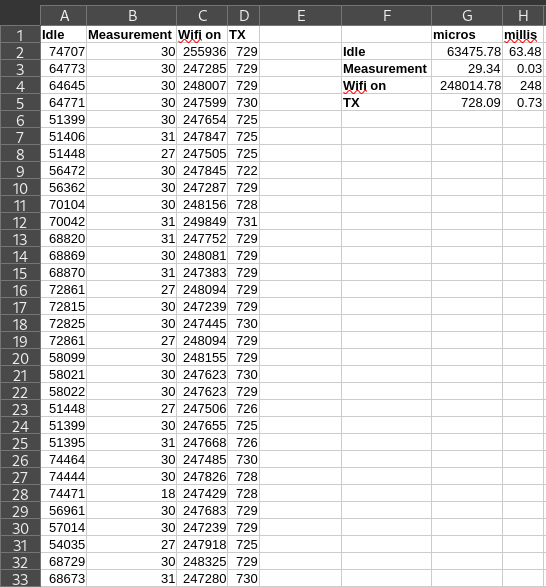
\includegraphics[width=\textwidth, height=0.71\textheight]{Images/state_duration.png}

\newpage
\section{Energy Consumption}
The energy consumption in each state is determined by multiplying the power consumption by the duration of that state:
\begin{itemize}
    \item transmission at 19dBm: $E_{TX} =1221,76$ $mW$ $*$ $728,1$ $\mu s$ $=$ $889,56$ $\mu J$
    \item sensor reading: $E_{SR} =466,74$ $mW$ $*$ $29,34$ $\mu s$ $=$ $13,69$ $\mu J$
    \item deep sleep: $E_{DS} =59,66$ $mW$ $*$ $41$ $s$ $=$ $2,45$ $J$ \\ (the deep sleep state lasts 41 seconds as specified in the project instructions)
    \item idle: $E_I =310,88$ $mW$ $*$ $63,48$ $ms$ $=$ $19,73$ $mJ$
    \item wifi on: $E_W =776,62$ $mW$ $*$ $248$ $ms$ $=$ $192,6$ $mJ$
\end{itemize}

Summing up all contributions, the total energy consumed per transmission cycle is:

$E = E_{DS}+E_{I}+E_{SR}+E_{W}+E_{TX}=2,66$ $J$

The sensor node is powered by a battery with an energy capacity of: \\ $(2886\mod 5000)+15000=17886$ $J$

The number of transmission cycles the battery can sustain is: $\frac{17886}{2,66}=6724$

Since the deep sleep state (41 $s$) is significantly longer than the other time intervals, we approximate the total battery life as: $6724*41s=275684$ $s\approx 76$ hours.

\section{Duty Cycle}
The following is an estimation of the duty cycle of the sensor given all of the previous durations and power consumptions of each state:\\
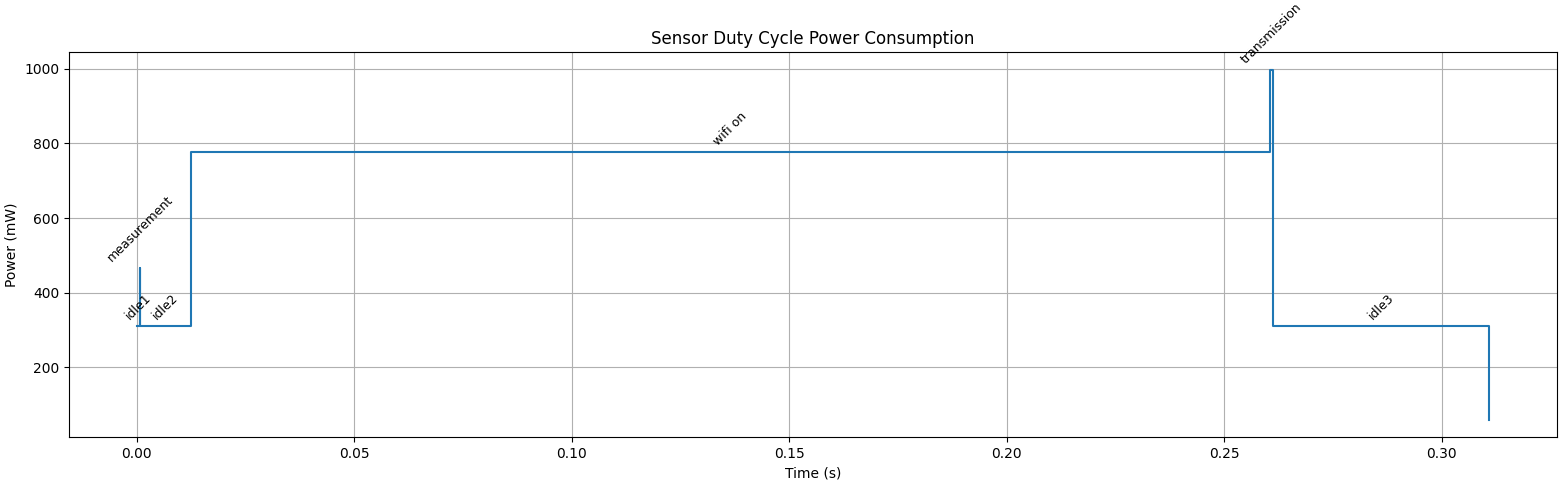
\includegraphics[width=\textwidth]{Images/duty_cycle.png}

\chapter{Improvements}
\label{ch:improvements}%

\section{Deep Sleep Optimization}
One effective way to extend the sensor node’s battery life is by increasing the duration of its deep sleep state. 

Using the previous formulas, we can plot battery lifetime against deep sleep duration. The results clearly show that beyond 90 seconds of deep sleep, any further increase provides negligible improvement in battery life.\\
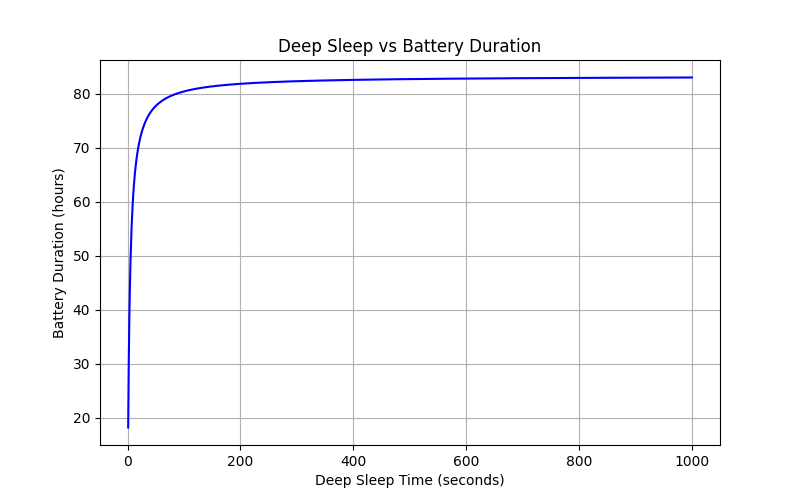
\includegraphics[width=\textwidth]{Images/deep sleep hours.png}

\newpage
Python script used to generate the plot:
\lstinputlisting[style=pythonStyle]{docs/stats/time.py}

Increasing the deep sleep duration to 90 seconds provides a battery life improvement. This duration also maintains an acceptable balance between energy efficiency and real-time system responsiveness. Increasing deep sleep to two minutes or more offers only marginal battery gains while potentially compromising the system’s real-time effectiveness.

Energy consumption in the case of 90 seconds of deep sleep:\\
$E_{DS} =59,66$ $mW$ $*$ $90$ $s$ $=$ $5,37$ $J$ \\
Hence the total energy consumed per transmission cycle is:\\
$E = E_{DS}+E_{I}+E_{SR}+E_{W}+E_{TX}=5,6$ $J$ 

The number of transmission cycles the battery can sustain is: $\frac{17886}{5,6}=3193$, using the same approximation as before, the total battery life is: $3193*90s\approx 79$ hours.


\section{Efficient Status Reporting}

Since increasing the deep sleep duration provides only a slight improvement in battery life, it may not be the most effective optimization. Instead, a better approach is to enhance the sensor node's energy efficiency reducing unnecessary Wi-Fi usage by utilizing RTC memory to store the last recorded status of the parking spot. 

The updated duty cycle will be as follows:
\begin{enumerate}
    \item the ultrasonic sensor will measure the distance to determine if the parking spot is OCCUPIED or FREE
    \item the new status will be compared to the last recorded status stored in RTC memory
    \item if the status remains unchanged, the node will skip Wi-Fi activation and return to deep sleep immediately
    \item if the status has changed, the node will turn on the WiFi, initialize the ESP-NOW communication, transmit the updated status to the sink node and finally turn the WiFi off before entering deep sleep
\end{enumerate}
The sink node will operate under the assumption that each parking spot is in the last reported state. It will only receive notifications when a change in status occurs, rather than receiving updates at fixed 41-second intervals.

I measured the average duration of each state, and the results closely match those from Chapter 2. The key difference is that if the parking spot's status remains unchanged, the device avoids Wi-Fi activation and transmission, reducing power consumption. 

In the worst case, where the parking spot changes status every 41 seconds, the estimated battery life remains the same as in Chapter 2 (approximately 76 hours). However, in more realistic scenarios where the status remains unchanged for multiple cycles, the battery will last longer.

If, for example, we assume that the status changes with a probability of 50\%, only half of the cycles will use the total energy needed which was $2,66J$, the other half will only consume $E_{SR}+E_{DS}+E_I=2,47J$\\
To compute the number $x$ of cycles that will drain the battery:\\
$2,66*x*0.5+2.47*x*0.5=17886$\\
$x = \frac{17886}{0.5*(2,47+2,66)}=6973$ cycles, which means the battery will last $6973*41s\approx 79$ hours.

If the probability of changing status is less than 50\%, then the lifetime of the battery will increase.

\subsection{Simulation}

Another \underline{\href{https://wokwi.com/projects/425676146192933889}{Wokwi project}} is available to simulate the new behaviour.

I used RTC\_NOINIT\_ATTR instead of RTC\_DATA\_ATTR because the latter does not retain its stored value during simulation, in this way the simulation resembles more the behaviour that the sensor would have if it were actually running.

\subsection{Duty Cycle}
The following is an estimation of the duty cycle of the sensor given all of the previous durations and power consumptions of each state in the case that the status doesn't change and there is no wifi and transmission states:\\ \\
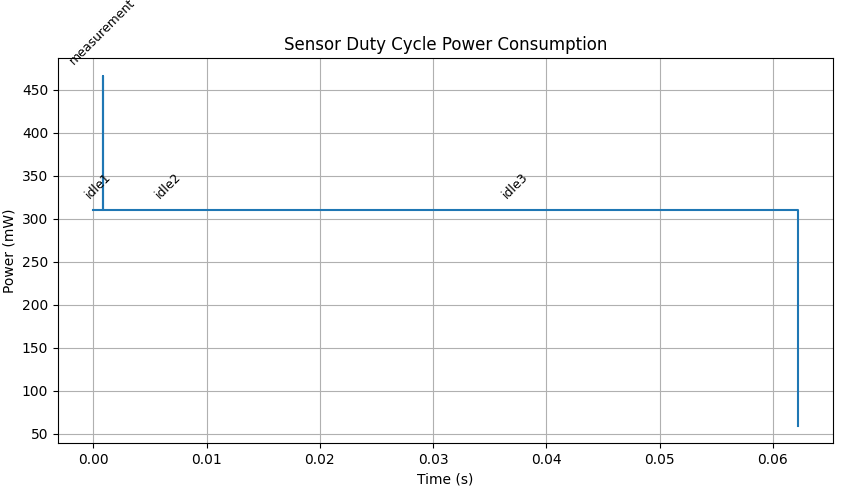
\includegraphics[width=\textwidth]{Images/opt_duty_cycle.png}

\cleardoublepage

\end{document}
